\section{Probabilitic Degree-based De-anonymization}
In this section, we describe the threat of node re-identification in uncertain graph data, and we explain the content of external information and the use of external information in identifying anonymized individual. We develop the intuition behind achieving anonymity in an uncertain graph through structural similarity to others. 

Here, we remind the reader its difference compared to the deterministic case. The incorporation of uncertainty in the graph data significantly affects the distribution of vertex property. Existing graph perturbation techniques are not equipped to operate over uncertain graphs -- they will tend to ignore and destroy important structural properties. Likewise, uncertain graph structure and adversary knowledge with an incorporation of uncertainty to threaten privacy in new ways. 

\begin{figure}[t!]
    \centering 
    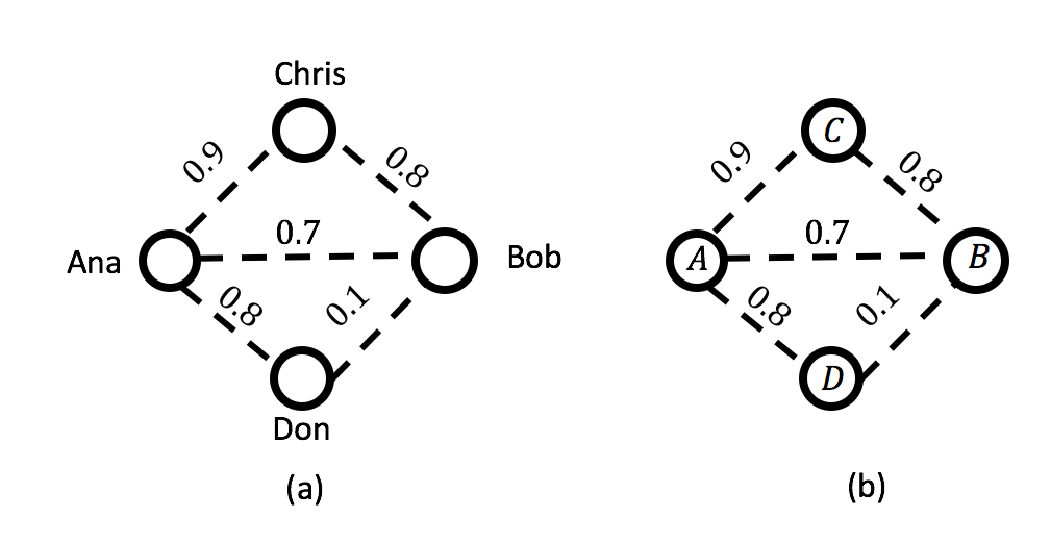
\includegraphics[scale=0.5]{figures/DegreeDistAUG/uncertainExample.eps}
    \caption{\small{(a) The original uncertain graph (b) The naive anonymized version of uncertain graph with 5 edges and $2^{5}=32$ possible world}}
    \label{fig:ddAUG:uncertainGraph}
\end{figure}

To gain more intuition on this attack model and the difficulties in defining a meaningful probabilistic matching, we present a simple example. Consider the original uncertain graph and the anonymized version of the given graph shown in Figure~\ref{fig:ddAUG:uncertainGraph}. We assume the adversary is equipped with the external structural information about some victim nodes. In particular, the property is node degree. Similarly, the degree of any nodes in the anonymized uncertain graph can be expressed as uncertain data. In the case of uncertain graph de-anonymization, the uncertainty belongs to the representation of source objects which are being identified, and the actual assertion is also probabilistic. In other words, fixed the node $v$ in the input uncertain graph, each node $u$ in the anonymized graph has a degree of being the image of $v$, which is probabilistic in nature. Meanwhile, the matching assertion is done by comparing two probability objects. 

\subsection{Adversary Knowledge}
We proceed to present the formal definition. Let us consider the knowledge that an adversary may extract from an uncertain graph about a given target vertex in $\mathcal{G}$. Following the literature, we assume that the adversary knows some vertex property $P$. In this work, we assume such property $P$ is the degree. Given an uncertain graph $\mathcal{G}$, each $v \in \mathcal{G}$ and the degree value $\omega$, we define the probability that $X_{v}(\omega)$ that $v$ originated from a vertex in $G$ with property value $\omega$. Specifically, 
\begin{equation*}
    X_{v}(\omega) = \sum_{G \in W(\mathcal{G})}  Pr(G) \cdot \mathcal{X}_{v,\omega}(G)
\end{equation*}
where $Pr(G)$ is the probability that the possible world $G$ is observed, and $\mathcal{X}_{v,w}(G)$ is 0-1 variable that indicates the vertex $v$ has the degree value $\omega$ in the possible world $G$. In other world, $X_{v}(\omega)$ is the sum of probabilites of all possibel worlds in which the vertex $v$ has the given property value $\omega$. We define the degree value of a node $v$ in an uncertain graph $d_{v}$ as an random variable with a probability distribution $X_{v}$. The probabilties $X_{v}(\omega)$ may be arrange in a $n \times |\Omega|$ matrix, where each row corresponding to one vertex $v in \mathcal{G}$ and it gives the probability distribution $X_{v}$. 
 \begin{table}[t!]
     \centering
      \begin{tabular}{|L{1.25cm}|c|c|c|c|}
             \cline{1-5}
                $\mathbf{X}_{v}(\omega)$ & $\text{deg}=0$ & $\text{deg}=1$ & $\text{deg}=2$ & $\text{deg}=3$ \\ \hline 
              $a$   & $0.006$ & $0.092$ & $0.398$ & $0.504$ \\ 
              $b$   & $0.054$ & $0.348$ & $0.542$ & $0.056$  \\
              $c$   & $0.020$ & $0.260$ & $0.720$ & $0.000$ \\
              $d$   & $0.180$ & $0.740$ & $0.080$ & $0.000$  \\  \hline 
 %              $\mathbf{S(\omega)}$   & $0.260$ & $1.440$ & $1.740$ & $0.560$ \\ \hline 
      \end{tabular} 
      \caption{The matrix $X_{v}(\omega)$ for the uncertain graph in Figure~\ref{fig:ddAUG:uncertainGraph} and the degree property.}
     \label{tab:DegreeMatrix}
 \end{table}


\begin{example}
    Consider the uncertain graph in Figure~\ref{fig:ddAUG:uncertainGraph} and assume the vertex property is degree. Table \ref{tab:DegreeMatrix} gives the corrsponding matrix $X_{v}(\omega)$, in which each row gives the probability distribution regrading the dgree of the corresponding vertex in $\mathcal{G}$. For instance, the probability that $a$ has degree $3$ is $0.9 \cdot 0.7 \cdot 0.8=0.504$. 
\end{example}

\subsection{Re-identification Attack}
The degree value of a node $u$ in the anonymized uncertain graph is defined as the corresponding random variable $d_{u}$.  The matching assertion is evaluated as the probability of the event two random variable $d_{u}$ and $d_{v}$ is equal. Specifically, 
\begin{align*}
    F_{u}(v)=P(d_{u}=d_{v})&=\sum_{\omega} P(d_{u}=\omega) \cdot P(d_{u}=\omega) \\
                  &=\sum_{\omega} X_{v}(\omega) \cdot X_{u}(\omega)
\end{align*}
The probabilities $F_{u}^{v}$ may be arrange in a $n \times n$ matrix, where each row corresponds to one vertex $u \in \tilde{\mathcal{G}}$ and it gives the corresponding probability $F_{u}^{v}$ over all possible target nodes $v \in V_{\mathcal{G}}$. The columns of that matrix are proportional to the probability distribution that correponding to victim nodes. More precisely, the normalized column corresponding to a target node $v$, {\ie}, 
\begin{equation*}
    Y_{v}(u):=\frac{F_{u}(v)}{\sum_{u \in \tilde{G}} F_{u}^{v}}
\end{equation*}
is the probability that $u$ is the image in $\tilde{\mathcal{G}}$ of a vertex that had property $d_{v}$ in $\mathcal{G}$.

 \begin{table}[t!]
     \centering
    \begin{tabular}{|L{1.25cm}|c|c|c|c|}
      \cline{1-5}
      $\mathbf{F_{u}^{v}}}$ & $v_{a}$ & $v_{b}$  & $v_{c}$ & $v_{d}$ \\ \hline 
      $u_{a}$ & 0.42092 & 0.27628 & 0.3106  &  0.101 \\
      $u_{b}$ & 0.27628 & 0.42092 & 0.4818 &  0.3106 \\
      $u_{c}$ & 0.3106  & 0.4818  & 0.5864 &  0.2536 \\
      $u_{d}$ & 0.101   & 0.3106  & 0.2536 &  0.5864 \\  \hline 
    \end{tabular}
    \caption{The matrix $F_{u}^{v}$ for the uncertain graph and itself in Figure~\ref{fig:ddAUG:uncertainGraph} and the degree property.}
    \label{tab:DegreeDistMatching}
 \end{table}


 \begin{table}[t!]
     \centering
    \begin{tabular}{|L{1.25cm}|c|c|c|c|}
      \cline{1-5}
      $\mathbf{Y_{u}^{v}}}$ & $v_{a}$ & $v_{b}$  & $v_{c}$ & $v_{d}$ \\ \hline 
      $u_{a}$ & 0.37962     & 0.18548  & 0.19027  &  0.08069 \\
      $u_{b}$ & 0.24917     & 0.28257  & 0.29515  &  0.24816 \\
      $u_{c}$ & 0.28012     & 0.32344  & 0.35922  &  0.20262 \\
      $u_{d}$ & 0.09109     & 0.20851  & 0.15535  &  0.46852 \\  \hline 
    \end{tabular}
    \caption{The matrix $Y_{u}^{v}$ for the uncertain graph and itself in Figure~\ref{fig:ddAUG:uncertainGraph} and the degree property.}
    \label{tab:DegreeDistPreimage}
 \end{table}

\begin{example}
    For example, if in the anonymization process we do nothing, then the perturbed output $\tilde{\mathcal{G}}=1$. In the case, the probability matrix induced by $\tilde{\mathcal{G}}$ equals to the one induced by $\mathcal{G}$. Table \ref{tab:DegreeDistMatching} gives the corresponding matrix $F$. For instance, the probability that $d_{a}$ is equal to $d_{c}$ is $0.006 \cdot 0.02 + 0.092 \cdot 0.26 + 0.398 \cdot 0.72 + 0.504 \cdot 0=0.3106$. After normalization them, give the corresponding $Y_{u}(v)$  distributions for each vertex $v$ in Table \ref{tab:DegreeDistPreimage}. For instance, if we look for a vertex that has the same degree distribution of $Ana$ in $\mathcal{G}$, it is either $a$, with probability around $0.38$, $b$ with probability around $0.25$, $c$ with probability around $0.28$, or $d$ with probability around $0.09$. 
\end{example}

\subsection{Privacy Notation}
Likewise, we can define our notion of privacy . 
\begin{definition}
    \textbf{\boldmath{$(k,\epsilon)$}-obf \cite{Bonchi_Identity_2014}}
    Let $P$ be the degree distribution, $k \geq 1$ be a desired level of anonymity, and $\epsilon >0 $ be a tolerance parameter. The uncertain graph $\tilde{\mathcal{G}}$ is said to $k$-obfuscate a given vertex $v \in V_{\mathcal{G}}$ with respect to $P$ if the entropy of the distribution $Y_{v}$ over the vertices of $\mathcal{G}$ is greater than or equals to $\log_{2}{k}$:
    \vj
    \begin{equation*}
        H(Y_{v}) \geq \log_{2}{k}.
    \label{obfCon}
    \svj
    \end{equation*}
The uncertain graph $\mathcal{G}$ is $(k,\epsilon)$-obf with respect to property $P$ if it $k$-obfuscates at least $(1-\epsilon)|V|$ vertices in $V_{\mathcal{G}}$. $P$ can be any node properties.  
\end{definition}
Namely, given the considered attack scenario, in which the adversary uses the degree distribution information of his target vertex $v$, we wish to lower bound the entropy of the distribution it induced over the perturbed graph vertices by $\log_{2}{k}$. The general idea is exact the same with {\keobf}, proposed in the literture~\cite{Bonchi_Identity_2014}. We extend the concept of equivalent class to probabilitic scenerio. 